\documentclass[a4paper,10pt]{article}
\usepackage[utf8]{inputenc}
\usepackage[english]{babel}
\usepackage{indentfirst}
\usepackage{listings}
\usepackage{graphicx}
\usepackage{blindtext}
\usepackage{enumitem}
\usepackage{hyperref}
\usepackage[top=2.5cm,bottom=2.5cm,left=2.5cm,right=2.5cm]{geometry}
\pagestyle{headings}
\title{Ftp server in a datadiode}
\author{Rusu George, Boulif Ilias, Orinx Cédric}
\date{\today}

\begin{document}
\maketitle
\newpage
\tableofcontents
\newpage
\section{Concept of operations}
\subsection{Introduction to the problem}
Our client would want to prevent his research and development labs against industrial espionage. He wants to divide the company network in order to maintain every lab in an isolated environment. Thus, the critical data could not leave the company labs using the network. One problem related is assuring that all the operating systems are up to date. This could be achieved using a manual operation where an employee would manually update every node in the isolated network using a mass-storage device\footnote{A USB-key for instance.}. However, this is not the most optimized way and for sure it is not cost less and timeless for the company without mentioning that there could be dependency problems, this is prone to human errors and this could generate security vulnerabilities.

\subsection{Our solution}
In order to address this problem we are going to implement a data diode. In electronics as shown in Figure \ref{fig:diode}, a diode is a component which conduct the current in one direction. Thus the term of data diode is something that only let the data to travel in an unidirectional way. An example of use case is illustrated in Figure \ref{fig:datadiode}, letting the data pass from a low risk VLAN\footnote{IEEE 802.1Q.} to a high risk VLAN but not the way around.
\begin{figure}
\centering
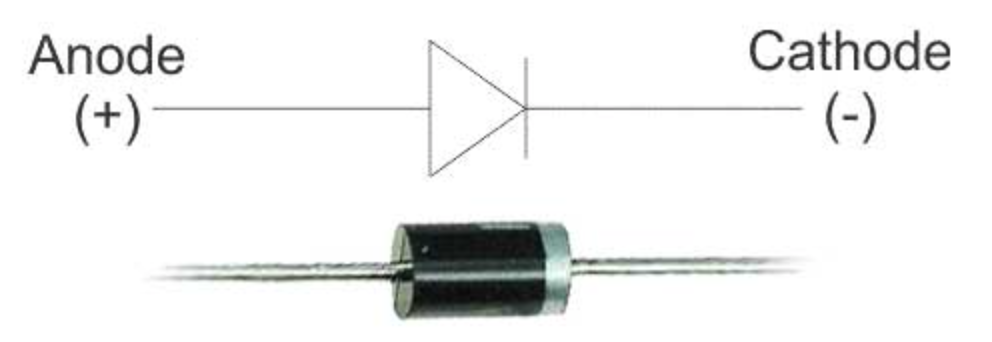
\includegraphics[scale=0.25]{images/diode.png}
\caption{A diode schema in electrionics.}
\label{fig:diode}
\end{figure}

\begin{figure}
\centering
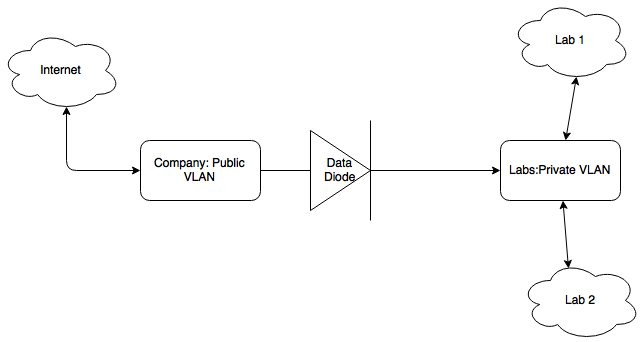
\includegraphics[scale=0.45]{images/dataDiode.png}
\caption{The schema of the usage of a data diode in a company network.}
\label{fig:datadiode}
\end{figure}

A data diode is made using a transmitter and a receiver both linked using one fiber cable. Thus when a digital data want to be send trough, every bit will be converted\footnote{using a Digital to analog converter (DAC).} into an electrical pulse that the transmitter will convert in light pulse using a LED\footnote{Light Emitting Diode.}. Then, the output light will pass trough the fiber cable and as soon as the photons are reaching the receiver, they will be reconverted firstly into a electrical pulse by a photo diode and then in bits\footnote{using an analog to digital converter (ADC).}.

One major problem is the network transport protocols(layer 4 in the OSI model) that applications are using. The most used transportation protocol is TCP. However, TCP is a bi-directional protocol which means that in order to start a connection there must be at leaste to fiber cable(the 3 ways handshake). Therefore, only UDP protocol can be used. TO BE CONTINUED 
\begin{figure}
\centering
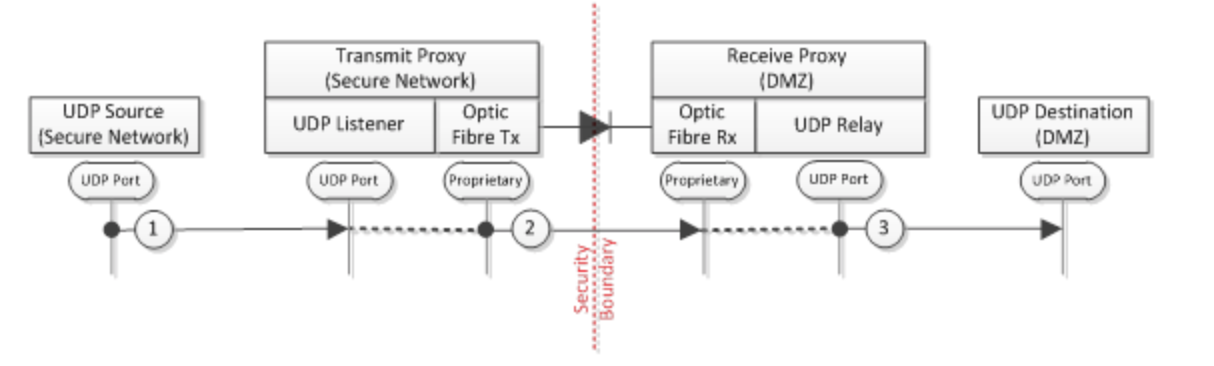
\includegraphics[scale=0.5]{images/UDPOverDD.png}
\label{fig:UDPDD}
\caption{UDP over a data diode.}
\end{figure}


\subsection{Our System implementation description}
The data diode concept is well orchestrated combination between hardware and software.
\subsubsection{Hardware}
\subsubsection{Software}
\subsubsection{Objectives}
\subsection{User Interface}
\subsection{System implementation}
\subsection{General usage}


\begin{thebibliography}{9}

\bibitem{nist-fips-202}
NIST,
\textit{SHA-3 Standard: Permutation-Based Hash and Extendable-Output Functions},
FEDERAL INFORMATION PROCESSING STANDARDS PUBLICATION,
2015.

\end{thebibliography}
\end{document}